We call \soset{} the pool of (concrete) solvers we plan to use in parallel to solve a problem. Once we have our solvers set, the last stage is to connect the solvers each others. Up to here, solvers are disconnected, but they have everything to establish the communication. \posl{} provides to the user a platform to easily define cooperative strategies that solvers must follow.

Following, we present two important concepts before we can formalize the {\it communication operators}.

\begin{definition}\label{def:comm_jack}
{\bf (Communication Jack)} Let a solver $\mathcal{S}$ be. Then, the operation $\mathcal{S}\cdot\mathcal{M}$ opens an outgoing connection from the solver $\mathcal{S}$ sending to the outside either 
\begin{inparaenum}[a)]
	\item the output of $\mathcal{M}$ if it is affected by a {\it sending data operator} presented in Definition~\ref{op:osend}, or
	\item $\mathcal{M}$ itself, if it is affected by a {\it sending module operator} presented in Definition~\ref{op:msend}.
\end{inparaenum}
\end{definition} 

\begin{definition}\label{def:comm_outlet}
{\bf (Communication Outlet)} Let a solver $\mathcal{S}$ be. Then, the operation $\mathcal{S}\cdot\mathcal{CM}$ opens an ingoing connection to the solver $\mathcal{S}$ receiving from the outside either 
\begin{inparaenum}[a)]
	\item the output of some \om{} if $\mathcal{CM}$ is a {\it data} \opch{}, or
	\item a \om{} if $\mathcal{CM}$ is an {\it object} \opch.
\end{inparaenum}
\end{definition} 


The communication is established by following the next rules guideline:
\begin{enumerate}%\begin{inparaenum}
	\item Each time a solver sends any kind of information by using a {\it sending} operator, it creates a \jack.
	\item Each time a solver defines a \opch, it creates a \outlet. 
	\item Solvers can be connected each others by linking \jacks{} to \outlets.
\end{enumerate} %\end{inparaenum}

%With the operator $(\cdot)$ we can have access to \oms{} sending information and to the \opch's names in a solver. 
%For example: $Solver_0\cdot \mathcal{M}$ provides access to the \om{} $\mathcal{M}$ in $Solver_0$ if and only if it is affected by a {\it sending} operator, and $Solver_1\cdot CM$ provides access to the \opch{} $CM$ in $Solver_1$.

Following, we define the \textit{connection operators} that \posl{} provides.

\begin{definition}\label{op_conn:1to1}
{\bf (Connection Operator One-to-One)} Let 
\begin{enumerate}
\item the list $\mathcal{J} = \left[\mathcal{S}_0\cdot \mathcal{M}_0, \mathcal{S}_1\cdot \mathcal{M}_1,\dots, \mathcal{S}_{N-1}\cdot \mathcal{M}_{N-1}\right]$ of \jacks, and
\item the list $\mathcal{O} = \left[\mathcal{Z}_0\cdot \mathcal{CM}_0, \mathcal{Z}_1\cdot \mathcal{CM}_1,\dots, \mathcal{Z}_{N-1}\cdot \mathcal{CM}_{N-1}\right]$ of \outlets{}
\end{enumerate} be. Then, the operation 
\[
\mathcal{J} \poslop{\rightarrow} \mathcal{O}
\]
Connects each \jack{} $\mathcal{S}_i\cdot \mathcal{M}_i \in \mathcal{J}$ with the corresponding \outlet{} $\mathcal{Z}_i\cdot \mathcal{CM}_i \in \mathcal{O}$, $\forall 0 \leq i \leq N-1$ (see Figure~\ref{subfig:comm_simple}).
\end{definition}

\begin{definition}\label{op_conn:1ton}
{\bf (Connection Operator One-to-N)} Let 
\begin{enumerate} 
\item the list $\mathcal{J} = \left[\mathcal{S}_0\cdot \mathcal{M}_0, \mathcal{S}_1\cdot \mathcal{M}_1,\dots, \mathcal{S}_{N-1}\cdot \mathcal{M}_{N-1}\right]$ of \jacks, and 
\item the list $\mathcal{O} = \left[\mathcal{Z}_0\cdot \mathcal{CM}_0, \mathcal{Z}_1\cdot \mathcal{CM}_1,\dots, \mathcal{Z}_{M-1}\cdot \mathcal{CM}_{M-1}\right]$ of \outlets{} 
\end{enumerate} be. Then, the operation 
\[
\mathcal{J} \poslop{\rightsquigarrow} \mathcal{O}
\]
Connects each \jack{} $\mathcal{S}_i\cdot \mathcal{M}_i \in \mathcal{J}$ with every \outlet{} $\mathcal{Z}_j\cdot \mathcal{CM}_j \in \mathcal{O}$, $\forall 0 \leq i \leq N-1$ and $0 \leq j \leq M-1$ (see Figure~\ref{subfig:comm_diff}).
\end{definition}

\begin{definition}\label{op_conn:ring}
{\bf (Connection Operator Ring)} Let 
\begin{enumerate} 
\item the list $\mathcal{J} = \left[\mathcal{S}_0\cdot \mathcal{M}_0, \mathcal{S}_1\cdot \mathcal{M}_1,\dots, \mathcal{S}_{N-1}\cdot \mathcal{M}_{N-1}\right]$ of \jacks, and 
\item the list $\mathcal{O} = \left[\mathcal{S}_0\cdot \mathcal{CM}_0, \mathcal{S}_1\cdot \mathcal{CM}_1,\dots, \mathcal{S}_{N-1}\cdot \mathcal{CM}_{N-1}\right]$ of \outlets{} 
\end{enumerate} be. Then, the operation 
\[
\mathcal{J} \poslop{\leftrightarrow} \mathcal{O}
\]
Connects each \jack{} $\mathcal{S}_i\cdot \mathcal{M}_i \in \mathcal{J}$ with the corresponding \outlet{} $\mathcal{Z}_{(i+1)\%N}\cdot \mathcal{CM}_{(i+1)\%N} \in \mathcal{O}$, $\forall 0 \leq i \leq N-1$  (see Figure~\ref{subfig:comm_ring}).
\end{definition}

\begin{figure}[h]
\centering
\subfloat[][Communication 1 to 1]{
	\label{subfig:comm_simple}
	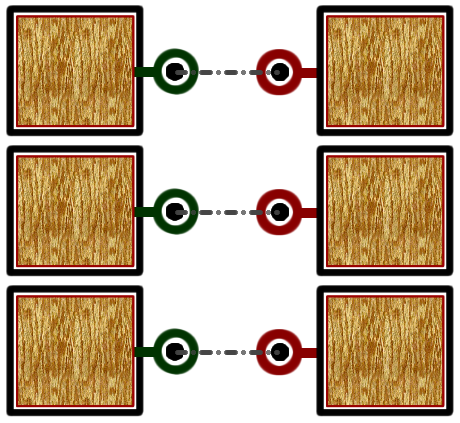
\includegraphics[width=0.25\textwidth]{comm_11.png}
}
\hspace{0.05\textwidth}%
\subfloat[][Communication 1 to N]{%
	\label{subfig:comm_diff}
	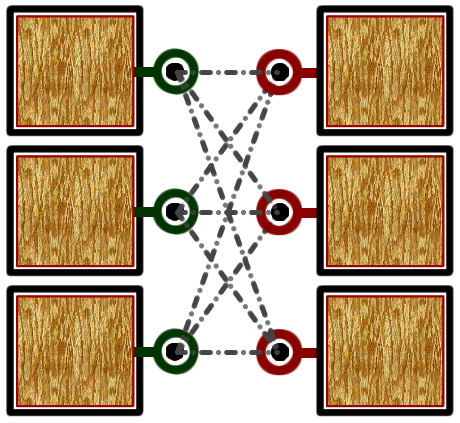
\includegraphics[width=0.25\textwidth]{comm_1n.png}
}
\hspace{0.05\textwidth}%
\subfloat[][Cyclic communication]{%
	\label{subfig:comm_ring}
	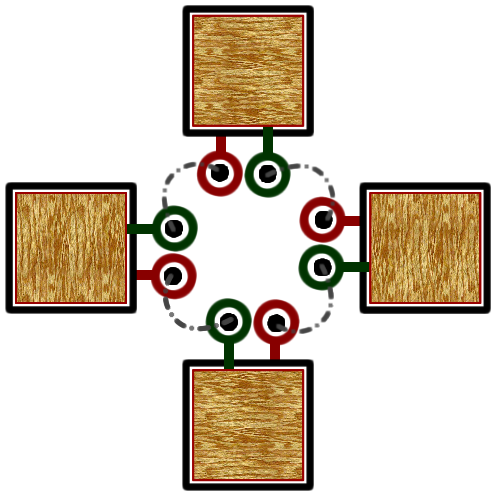
\includegraphics[width=0.25\textwidth]{comm_ring2.png}
}
\caption[]{Graphic representation of communication operators}
\label{fig:comm}
\end{figure}

\modified{\posl{} allows also declare not communicating solvers to be executed in parallel, declaring only the list of solvers names:}
\[
\left[\mathcal{S}_0, \mathcal{S}_1, \dots, \mathcal{S}_{N-1}\right]
\]


\modified{When we apply a connection operator $\circled{op}$ between a \jacks{} list $\mathcal{J}$ and a \outlets{} list $\mathcal{O}$, internally we are assigning an \textit{abstract computation unit} (typically a thread) to each solver that we declare in each list. This assignation receives the name of \textit{Solver Scheduling}. Before running the \soset{} this \textit{abstract unit of computation} is just an integer $\tau \in [0..N]$ as unique identifier for each solver. When the \soset{} is launched, the solver with the identifier $\tau$ runs into the computation unit $\tau$. This identifier assignation remains independent of the real availability of resources of computation. It just take into account the user declaration. It means that, if the user declares 30 solvers (15 senders and 15 receivers) and the \soset{} is launched using 20 cores, only the firsts 20 solvers will be executed, and in consequence, there will be 10 solvers sending information to nowhere. Users should take this into account at the time of declaring the \soset.}

\modified{The connection process depends on the applied conection operator. In each case the goal is to assign to the sending operator ($\llparenthesis .\rrparenthesis^{o}$ or $\llparenthesis .\rrparenthesis^{m}$) into the \as{}, the identifier of the solver (or solvers, depending on the connection operator) where the information will be sent. Algorithm~\ref{algo:connecting} presents the connection process.}

\incmargin{1.4em}
\linesnumbered
\begin{algorithm}[H]
\dontprintsemicolon
\SetLine
\SetKwFor{While}{while}{do}{end}
\SetKwData{Jacks}{$\mathcal{J}$}
\SetKwData{Outlets}{$\mathcal{O}$}
\SetKwData{SS}{$S$}
\SetKwData{SSjack}{$S_{jack}$}
\SetKwData{RR}{$R$}
\SetKwData{RRoutlet}{$R_{oulet}$}
\SetKwData{RRid}{$R_{id}$}
\SetKwFunction{GetSolver}{GetSolverFromConnector}
\SetKwFunction{GetNext}{GetNext}
\SetKwFunction{Sched}{Schedule}
\SetKwFunction{Root}{root}
\SetKwFunction{Connect}{Connect}
\SetKwInOut{Input}{input}
\SetKwInOut{Output}{output}
\SetKw{KwTo}{int}

\Input{\Jacks list of \jacks{}, \\ \Outlets list of \outlets}
%\Output{\Q = $\left\{Q_i\right\}_{i=1\dots K}$: $K$ subsets of \Uni}
%\BlankLine
\While{no available jacks or outlets}{ %\nllabel{paso_condicion}
	\SSjack	$\leftarrow$ \GetNext{\Jacks}\;
	\RRoutlet $\leftarrow$ \GetNext{\Outlets}\;
	\SS $\leftarrow$ \GetSolver{\SSjack}\;	
	\RR $\leftarrow$ \GetSolver{\RRoutlet}\;
	\Sched{\SS}\;
	\RRid $\leftarrow$ \Sched{\RR}\;
	\Connect{\Root{\SS},\SSjack, \RRid} %\label{step2} \tcc{It also removes the returned element}
}
\caption{Scheduling and connection main algorithm}\label{algo:connecting}
\end{algorithm}

In Algorithm~\ref{algo:connecting}:
\begin{itemize}
\item \texttt{GetNext($\dots$)} Returns the next available solver-jack (or solver-outlet) in the list, depending on the connection operator, e.g., for the connection operator One-to-N, each \jack{} in $\mathcal{J}$ must be connected with each \outlet{} in $\mathcal{O}$.
\item \texttt{GetSolverFromConnector($\dots$)} Returns the solver name given a connector declaration.
\item \texttt{Schedule($\dots$)} Schedule a solver and returns its identifier.
\item \texttt{Root($\dots$)} Returns the {\it root} \cm{} of a solver.
\item \texttt{Connect($\dots$)} %is presented in Algorithm~\ref{algo:connect}. It 
Searches the \om{} $S_{jack}$ recursively inside the {\it root} \cm{} of $S$ and places the identifier $R_{id}$ into its list of destination solvers.
\end{itemize}

%\incmargin{1.4em}
%\linesnumbered
%\begin{algorithm}[H]
%\dontprintsemicolon
%\SetLine
%\SetKwFor{While}{while}{do}{end}
%\SetKwData{Jacks}{$\mathcal{J}$}
%\SetKwData{Outlets}{$\mathcal{O}$}
%\SetKwData{Mroot}{$M$}
%\SetKwData{MM}{$\eta$}
%\SetKwData{ID}{$R_{id}$}
%\SetKwData{OP}{$\circled{op}$}
%\SetKwFunction{Oper}{Operator}
%\SetKwFunction{Module}{ExtractModule}
%\SetKwFunction{Connect}{Connect}
%\SetKwInOut{Input}{input}
%\SetKwInOut{Output}{output}
%
%\Input{\Mroot, \MM : \cms \\ \ID : integer}
%\If{\Mroot is an \operation}
%{
%	\OP $\leftarrow$ \Oper{\Mroot}\;
%	\If{$\circled{op} = \llparenthesis .\rrparenthesis^{o}\textbf{ OR } \circled{op} = \llparenthesis .\rrparenthesis^{m}$}
%	{
%		m = $\leftarrow$ \Module{\OP}\;
%		\If{ m $=$ \MM }{
%			Add \ID to the destinies list of \OP\;
%		}
%	}
%}{
%	\Conect{}
%}
%%\ElseIf{}{
%%all is wrong\;
%%\Return result52\;
%%}
%\caption{Scheduling and connection main algorithm}\label{algo:connect}
%\end{algorithm}

\subsection{Solver name space expansion}

\tet{Includeing an introduction here.}
\modified{\posl{} provides to ways of space name expansion:}

\textbf{Solver name expansion - } Using an integer $K$ to denote how many times the solver name $S$ will appear in the declaration. $\left[\dots S_i\cdot\mathcal{M}(K),\dots\right]$ expands as $\left[\dots S_i\cdot\mathcal{M}, S_i^2\cdot\mathcal{M},\dots S_i^K\cdot\mathcal{M}\dots\right]$\\
and all new solvers $S_i^j, j\in [2..K]$ are created using the same solver declaration of solver $S_i$.

\textbf{Connection declaration expansion - } Using an integer $K$ to denote how many times the connection will be repeated in the declaration. Let 
\begin{inparaenum}[a)]
\item the list $\left[\mathcal{S}_1\cdot\mathcal{M}_1,\dots,\mathcal{S}_{N}\cdot\mathcal{M}_{N}\right]$ of \jacks,
\item the list $\left[\mathcal{R}_1\cdot\mathcal{CM}_1,\dots,\mathcal{R}_{M}\cdot\mathcal{CM}_{M}\right]$ of \outlets{}, and
\item an connection operator $\circled{op}$
\end{inparaenum} be. Then, $$\left[\mathcal{S}_1\cdot\mathcal{M}_1,\dots,\mathcal{S}_{N}\cdot\mathcal{M}_{N}\right] \poslop{op} \left[\mathcal{R}_1\cdot\mathcal{CM}_1,\dots,\mathcal{R}_{M}\cdot\mathcal{CM}_{M}\right]K$$ expands as

\begin{align*}
\left[\mathcal{S}_1\cdot\mathcal{M}_1,\dots,\mathcal{S}_{N}\cdot\mathcal{M}_{N}\right] &\poslop{op} \left[\mathcal{R}_1\cdot\mathcal{CM}_1,\dots,\mathcal{R}_{N}\cdot\mathcal{CM}_{N}\right]\\
\left[\mathcal{S}_1^2\cdot\mathcal{M}_1,\dots,\mathcal{S}_{N}^2\cdot\mathcal{M}_{N}\right] &\poslop{op} \left[\mathcal{R}_1^2\cdot\mathcal{CM}_1,\dots,\mathcal{R}_{N}^2\cdot\mathcal{CM}_{N}\right]\\
&\dots\\
\left[\mathcal{S}_1^K\cdot\mathcal{M}_1,\dots,\mathcal{S}_{N}^K\cdot\mathcal{M}_{N}\right] &\poslop{op} \left[\mathcal{R}_1^K\cdot\mathcal{CM}_1,\dots,\mathcal{R}_{N}^K\cdot\mathcal{CM}_{N}\right]\\
\end{align*}
and all new solvers $S_i^k, i\in[1..N]$ and $R_j^k,j\in [1..M]$, with $k\in[2..K]$ are created using the same solver declaration of solvers $S_i$ and $R_j$ respectively.